\documentclass[11pt,a4paper]{article}

\usepackage[T1]{fontenc}
\usepackage{amsmath,amssymb,amsthm,mathtools}
\usepackage{booktabs}
\usepackage{enumitem}
\usepackage{graphicx}
\graphicspath{{../figures/}}
\usepackage[margin=2.4cm]{geometry}
\usepackage[colorlinks=true,linkcolor=blue,citecolor=blue,urlcolor=blue]{hyperref}
\usepackage{cleveref}

\newtheorem{theorem}{Theorem}[section]
\newtheorem{lemma}[theorem]{Lemma}
\newtheorem{proposition}[theorem]{Proposition}
\newtheorem{corollary}[theorem]{Corollary}
\theoremstyle{definition}
\newtheorem{definition}[theorem]{Definition}
\newtheorem{remark}[theorem]{Remark}
\newtheorem{conjecture}[theorem]{Conjecture}

\newcommand{\Pol}{\mathcal{P}}
\newcommand{\Zn}{\mathbb{Z}}
\newcommand{\Cat}{\mathrm{C}}
\newcommand{\TT}{\mathcal{T}}
\newcommand{\gap}{\mathrm{gap}}
\newcommand{\maxgap}{\mathrm{maxgap}}
\newcommand{\light}{\mathrm{light}}
\newcommand{\half}{\mathrm{half}}

\title{\bfseries The Triple-Covering Number of a Convex Polygon:\\
A Gap-Weight Certificate}
\author{}
\date{}

\begin{document}
\maketitle

\begin{abstract}
Let $\Pol_n$ be a convex $n$-gon. Call a family of triangulations of $\Pol_n$ a
\emph{triple cover} if every three-element subset of the vertices is a face of at
least one of its members, and let $T(n)$ be the minimum size of a triple cover.
We prove the sharp lower bound
\[
T(n)\ \ge\ \Phi(n) := \begin{cases}
2\binom(M+1,3), & n = 2M,\\[2pt]
\displaystyle\sum_{j=1}^{M} j^2, & n = 2M+1,
\end{cases}
\qquad (n \ge 5),
\]
and we determine $T(n)$ exactly for $3 \le n \le 14$, where in every case the
value equals $\Phi(n)$ and optimality is witnessed by a machine-checked
certificate. The bound is obtained from an explicit weight $y$ on triples,
defined through the largest cyclic gap between their vertices. The proof rests on
two clean structural facts about a single triangulation: any two of its faces
$F, G$ satisfy $\maxgap(F) + \maxgap(G) \ge n-2$ (\emph{Lemma~\ref{lem:gapsum}}),
and, when $n$ is even, all faces of weight $1/2$ contain one common antipodal
chord (\emph{Lemma~\ref{lem:antipodal}}). Together these imply that the faces of
any triangulation have total weight at most $1$, while a short
inclusion--exclusion computation shows that the total weight of all triples is
exactly $\Phi(n)$; double counting finishes the argument. As a by-product we
solve a sub-problem exactly: the $n$ fans cover every triple that uses a
boundary edge, each such triple exactly once, and $n$ is optimal for that
sub-problem. We conjecture $T(n) = \Phi(n)$ for all $n \ge 5$. Randomized greedy
set cover attains $\Phi(n)$ for $n \le 12$, but we do \emph{not} prove a general
construction; Section~\ref{sec:gap} is devoted to the honest analysis of what is
still missing. No prior result on triple covers of convex polygons was found; the
closest literature concerns book thickness and extremal families of triangles in
convex position, discussed in Section~\ref{sec:related}.
\end{abstract}

\section{Introduction}\label{sec:intro}

Covering all diagonals of a convex polygon by triangulations has a classical
answer: the diagonals of $\Pol_n$ can be partitioned into $\lceil n/2\rceil$
triangulations, and no fewer will do, since a triangulation has $n-3$ diagonals
and there are $n(n-3)/2$ of them. This is a repackaging of the book-thickness
theorem $\mathrm{bt}(K_n) = \lceil n/2\rceil$ of Bernhart and Kainen
\cite{bernhartkaainen1979}: we first attempted this direction and abandoned it
precisely because the lower bound is a one-line count and the upper bound is a
classical construction. That experience shaped the present paper, which asks a
strictly harder question in the same setting.

\begin{definition}[Triple cover]\label{def:triplecover}
Let $\Pol_n$ be the convex $n$-gon with vertex set $V = \Zn/n\Zn$ in cyclic order. A
family $\mathcal{F}$ of triangulations of $\Pol_n$ is a \emph{triple cover} if for
every $S \in \binom{V}{3}$ there is $T \in \mathcal{F}$ in which $S$ is a face.
Write
\[
T(n) = \min\{|\mathcal{F}| : \mathcal{F} \text{ is a triple cover of } \Pol_n\}.
\]
\end{definition}

The question ``how many triangulations does it take so that every inscribed
triangle appears?'' is a natural hybrid of two classical topics: the
decomposition of complete graphs into outerplanar pieces, and covering designs
with restricted blocks. Unlike the diagonal-covering problem, it is not
controlled by counting: a single triangulation carries only $n-2$ of the
$\binom{n}{3}$ triples, so counting gives $\binom{n}{3}/(n-2) = n(n-1)/6$, whereas
the true answer grows like $n^3/24$, a factor of roughly $n/4$ larger. This gap
is the mathematical content of the paper.

\paragraph{Results.}
\begin{itemize}[leftmargin=1.4em]
\item \textbf{Main theorem.} $T(n) \ge \Phi(n)$ for all $n \ge 5$, where
      $\Phi(2M) = 2\binom(M+1,3)$ and $\Phi(2M+1) = \sum_{j\le M} j^2$. Since
      $\Phi(n) = n^3/24 - O(n)$, this yields $T(n) = \Omega(n^3)$.
\item \textbf{Exact values.} $T(n) = \Phi(n)$ for $3 \le n \le 14$, each with a
      verified optimality certificate (the LP-dual optimum equals the integer
      optimum of the set-cover formulation).
\item \textbf{A solved sub-problem.} $n$ triangulations suffice to cover all
      triples that use at least one boundary edge, and $n$ is necessary.
\item \textbf{Structural lemmas.} The gap-sum bound $\maxgap(F) + \maxgap(G) \ge
      n-2$ for any two faces of a triangulation (tight), and the antipodal-chord
      description of the $1/2$-weight faces for even $n$.
\item \textbf{Conjecture.} $T(n) = \Phi(n)$ for all $n \ge 5$.
\end{itemize}

\paragraph{Method.} Assign to every triple $S$ a weight $y(S) \in \{0, \tfrac12, 1\}$
depending only on the largest cyclic gap between its vertices
(Definition~\ref{def:weight}). We prove that the faces of any single
triangulation have total weight at most $1$ (Theorem~\ref{thm:weightbound}); since
a family of $t$ triples covers has to pay $\sum_S y(S)$ in total, the bound
$T(n) \ge \sum_S y(S)$ follows, and the right-hand side is exactly $\Phi(n)$
(Lemma~\ref{lem:counting}). The computation of $\sum_S y(S)$ is a routine
inclusion--exclusion over compositions; the real work is the geometric
Lemma~\ref{lem:gapsum} and the parity-sensitive Lemma~\ref{lem:antipodal}.

\section{Related work and novelty}\label{sec:related}

\paragraph{Book thickness and geometric decompositions.}
A \emph{$p$-page book embedding} of a graph draws the vertices on a line and
partitions the edges into $p$ crossing-free outerplanar pages; the minimum $p$ is
the book thickness $\mathrm{bt}(G)$. Bernhart and Kainen proved
$\mathrm{bt}(K_n) = \lceil n/2\rceil$ \cite{bernhartkaainen1979}, and the
standard construction puts the vertices on a circle so that each page is a
triangulation of $\Pol_n$ together with the boundary cycle. Hence
\emph{every diagonal of $\Pol_n$ is used in one of $\lceil n/2\rceil$ triangulations,
and this is optimal.} Our first research direction was exactly this statement;
we rejected it because the lower bound $\lceil n(n-3)/2 / (n-3) \rceil =
\lceil n/2\rceil$ is immediate and the construction is classical. We mention it
because it is the closest relative of our problem and because the failure of the
counting argument there is precisely what makes the triple-covering problem
interesting.

The thickness of $K_n$ (Buchberger--Osipov \cite{buchbergerosipov1998}; see also
the survey of Beineke and Harary \cite{beinekeharary1965}) and the outerthickness
of $K_n$ are further classical decompositions into planar/outerplanar pieces.
Again, they concern edge partitions, not the covering of vertex triples by
triangulations.

\paragraph{Ears, dual trees, Catalan numbers.}
The number of triangulations of $\Pol_n$ is the Catalan number $\Cat_{n-2}$ (Euler),
a triangulation has $n-2$ faces and $n-3$ diagonals, and the classical two-ears
theorem says that a triangulation has at least two ears, where an ear is a face
using two boundary edges. These facts are used in
Proposition~\ref{prop:budget} and Proposition~\ref{prop:maxears}; we include
proofs to keep the paper self-contained.

\paragraph{Extremal families of triangles in convex position.}
Closest to the present work is the theory of convex geometric hypergraphs, in
particular the study of families of inscribed triangles that pairwise intersect.
Füredi, Mubayi, O'Neill and Verstraëte \cite{furedietal2020} determine the
extremal functions for all eight configurations consisting of two disjoint
triples, and in particular solve a problem of Frankl, Holmsen and Kupavskii on
the maximum size of an intersecting family of triangles of $n$ points in the
plane. Our \emph{light triples} are a different local constraint: a triple is
light when no cyclic gap exceeds $\lfloor (n-3)/2 \rfloor$, and
Lemma~\ref{lem:gapsum} says that two light triples can never be faces of the
same triangulation. We are not aware of this condition appearing in that
literature.

\paragraph{Covering designs.}
In the language of covering designs \cite{colbourndinitz} our problem is a
covering design in which the admissible blocks are exactly the face sets of
triangulations of a fixed $n$-gon, so that blocks are far more constrained than
arbitrary $3$-subsets. Standard covering-design lower bounds (the counting bound
$\binom{v}{t}/k$) are reproduced in Lemma~\ref{lem:capacity} and are far from
sufficient here.

\paragraph{Novelty statement.}
We did not find any published source that studies $T(n)$, the minimum number of
triangulations of a convex polygon needed to realise every vertex triple as a
face. We searched for it under the terms ``triple cover'', ``covering all
triangles by triangulations'', ``set cover with triangulation blocks'',
``covering designs on triangulations of a polygon'', and in convex geometric
hypergraph literature on intersecting families of inscribed triangles. The
structural lemmas of Section~\ref{sec:main} and the certificate construction are
ours; the individual ingredients (Catalan counts, the ear/dual-tree identity, the
two-ears bound) are classical and cited as such. We make no claim of priority
beyond this.

\section{Preliminaries}\label{sec:prelim}

Let $P_n$ be the convex polygon with vertices $\Zn/n\Zn$ in cyclic order; indices
are read modulo $n$. A \emph{boundary edge} is $\{i, i+1\}$. For a triple
$S = \{a, b, c\}$ written $a < b < c$ define its three cyclic \emph{gaps}
\begin{equation}\label{eq:gaps}
  g_1(S) = b - a - 1, \qquad g_2(S) = c - b - 1, \qquad g_3(S) = n - 1 - c + a,
\end{equation}
the numbers of vertices strictly between consecutive elements of $S$ around the
cycle, and put $\gap(S) = (g_1, g_2, g_3)$ and $\maxgap(S) = \max_i g_i(S)$.
Two elementary facts will be used constantly:
\begin{equation}\label{eq:gapsum}
  g_1 + g_2 + g_3 = n - 3 \quad \text{for every triple, and} \quad
  g_i(S) = 0 \iff \text{two elements of } S \text{ are adjacent}.
\end{equation}

\begin{definition}[Types of a triple]\label{def:types}
For $n \ge 5$ the type of a triple $S$ is $A$, $B$ or $C$ according as $S$ uses
two, one or zero boundary edges; equivalently, according as $\gap(S)$ has two,
one or no zero entries. We write $\mathcal{A}_n, \mathcal{B}_n, \mathcal{C}_n$ for
the three classes and $|\mathcal{A}_n| = n$, $|\mathcal{B}_n| = n(n-4)$,
$|\mathcal{C}_n| = n(n-4)(n-5)/6$.
\end{definition}

The counts in Definition~\ref{def:types} are immediate: there are $n$ triples of
type $A$ (three consecutive vertices); a triple of type $B$ is determined by a
boundary edge and a third vertex that is adjacent to neither endpoint, giving
$n \cdot (n-4)$ choices; the rest are of type $C$. We use $A$-, $B$- and
$C$-faces for the faces of a triangulation of the three types.

A \emph{triangulation} of $\Pol_n$ is a maximal set of pairwise non-crossing
diagonals; it has $n-3$ diagonals, $n-2$ faces, and the number of triangulations
is $\Cat_{n-2}$. The \emph{dual graph} of a triangulation has the faces as
vertices and joins two faces sharing a diagonal; it is a tree, and a face has
dual degree $2 - (\text{number of its boundary edges})$, i.e.\ degree $1$, $2$ or
$3$ for faces of type $A$, $B$, $C$ respectively.

\section{Structural facts}\label{sec:struct}

\begin{proposition}[Face budget]\label{prop:budget}
Let $T$ be a triangulation of $\Pol_n$ with $e$ ears, i.e.\ $e$ faces of type $A$.
Then the numbers of faces of type $A$, $B$, $C$ are
\[
(e,\ n - 2e,\ e - 2).
\]
Consequently $2 \le e \le \lfloor n/2 \rfloor$ and $T$ has at most
$\lfloor n/2 \rfloor - 2$ faces of type $C$.
\end{proposition}

\begin{proof}
A face of type $A$ uses two boundary edges, a face of type $B$ one, a face of
type $C$ none, and all $n$ boundary edges are used exactly once, so if the face
counts are $(\alpha, \beta, \gamma)$ then
\[
  2\alpha + \beta = n \qquad\text{and}\qquad \alpha + \beta + \gamma = n-2 .
\]
Taking $\alpha = e$ and solving gives $\beta = n - 2e$ and $\gamma = e - 2$; the
dual tree supplies no further equation, since $\alpha + 2\beta + 3\gamma = 2(n-3)$
follows from the two above. Since ears are pairwise non-adjacent vertices,
$e \le \lfloor n/2 \rfloor$; and $e \ge 2$ by the two-ears theorem.
\end{proof}

\begin{proposition}[Maximal ears are rare]\label{prop:maxears}
Let $I(n, m)$ be the number of independent $m$-sets of the cycle $\Cat_n$, so
$I(n, m) = \frac{n}{n-m}\binom{n-m}{m}$. The number of triangulations of $\Pol_n$ with
exactly $\lfloor n/2 \rfloor$ ears is
\[
I\!\left(n, \lfloor n/2 \rfloor\right) \cdot \Cat{\lceil n/2 \rceil - 2}.
\]
\end{proposition}

\begin{proof}
Let $E$ be the ear set. Removing the ears one at a time deletes $|E|$ vertices
and leaves a polygon on $n - |E|$ vertices which is triangulated arbitrarily.
If $|E| = \lfloor n/2 \rfloor$ then $n - |E| = \lceil n/2 \rceil$, and no ear of
the residual polygon would enlarge $E$ beyond $\lfloor n/2 \rfloor$, so the
construction is a bijection with triangulations of the residual
$\lceil n/2 \rceil$-gon, of which there are $\Cat{\lceil n/2 \rceil - 2}$.
\end{proof}

\begin{theorem}[The type-$A$/$B$ sub-problem]\label{thm:fan}
Let $F_v$ be the fan of $\Pol_n$ at the vertex $v$, i.e.\ the triangulation
consisting of all diagonals through $v$. Then $\{\mathcal{F}_v : v \in V\}$ covers
every $A$- and every $B$-triple, each exactly once, and no family of fewer than
$n$ triangulations covers all $B$-triples. Consequently the minimum number of
triangulations needed to cover all triples having a boundary edge equals $n$.
\end{theorem}

\begin{proof}
The faces of $\mathcal{F}_v$ are $\{v, v+i, v+i+1\}$ for $i = 1, \dots, n-2$, so
every $B$-triple $\{u, u+1, w\}$ is a face of $\mathcal{F}_w$ and of no other
fan; every $A$-triple is a face of the three fans at its vertices. There are
$|\mathcal{B}_n| = n(n-4)$ $B$-triples, and by Proposition~\ref{prop:budget} a
triangulation with $e \ge 2$ ears has $n - 2e \le n-4$ faces of type $B$, so any
cover of all $B$-triples needs at least $\lceil n(n-4)/(n-4) \rceil = n$ blocks.
\end{proof}

\section{The certificate}\label{sec:main}

\begin{definition}[Light and half triples; the weight]\label{def:weight}
Fix $n \ge 5$ and put $k = \lfloor (n-3)/2 \rfloor$. Call a triple $S$
\emph{light} if $\maxgap(S) \le k$ and \emph{half} if $\maxgap(S) = k + 1$.
Define
\[
y(S) = \begin{cases}
  1, & S \text{ light},\\
  \tfrac12, & S \text{ half and } n \text{ even},\\
  0, & \text{otherwise}.
\end{cases}
\]
\end{definition}

The two structural lemmas below are the heart of the argument.

\begin{lemma}[Gap-sum]\label{lem:gapsum}
Let $T$ be a triangulation of $\Pol_n$ and let $F \ne G$ be two of its faces. Then
$\maxgap(F) + \maxgap(G) \ge n - 2$. The bound is attained.
\end{lemma}

\begin{proof}
Faces of a triangulation have pairwise disjoint interiors. We distinguish the
three possibilities for $F$ and $G$. Note first that a gap of a triple is the
number of vertices strictly inside one of the three arcs determined by the
triple, so ``the arc opposite the third vertex'' is always one of the gaps.

\emph{(a) They share an edge $\{x, y\}$.} Let the third vertex of $F$ lie in the
arc with $u$ interior vertices and the third vertex of $G$ in the other arc, which
has $v$ interior vertices; $u + v = n - 2$. The arc of $F$ opposite its third
vertex is the second one, so $\maxgap(F) \ge v$, and symmetrically
$\maxgap(G) \ge u$. Hence $\maxgap(F) + \maxgap(G) \ge u + v = n-2$.

\emph{(b) They share exactly one vertex.} Rotate so the shared vertex is $0$ and
write $F = \{0, p, q\}$, $G = \{0, r, s\}$ with $0 < p < q < r < s$ (the wedges at
the shared vertex must be disjoint and unnested, otherwise the faces would
overlap). Then the arc from $q$ back to $0$ gives $\maxgap(F) \ge n-1-q$ and the
arc from $0$ to $r$ gives $\maxgap(G) \ge r - 1$, whence
$\maxgap(F) + \maxgap(G) \ge n - 2 + (r - q) \ge n-1$.

\emph{(c) They are disjoint.} Then one of them, say $G$, lies inside a single cap
of $F$, bounded by a diagonal of $F$; let that cap have $g$ interior vertices,
so $g$ is a gap of $F$ and $\maxgap(F) \ge g$, while the arc of $G$ around the
rest of the polygon has at least $n - 1 - g$ interior vertices, so
$\maxgap(G) \ge n - 1 - g$ and the sum is at least $n-1$.

In all cases the sum is at least $n-2$. Equality is realised, e.g. in $\Pol_5$ by
the faces $\{0,1,2\}$ and $\{0,2,3\}$, and verified exhaustively for $5 \le n
\le 12$ by the code \texttt{verify\_gap\_sum\_lemma}.
\end{proof}

\begin{lemma}[Antipodal chords]\label{lem:antipodal}
Let $n = 2M$ be even. Let $T$ be a triangulation of $\Pol_n$.
\begin{enumerate}[label=(\roman*)]
\item Every face $F$ with $\maxgap(F) = M-1$ contains a chord $\{v, v+M\}$
      joining antipodal vertices, and this chord is unique for $F$.
\item Two distinct faces with $\maxgap = M-1$ contain the same antipodal chord;
      consequently there are at most two such faces.
\item No face with $\maxgap \le M-2$ belongs to a triangulation that also has a
      face with $\maxgap = M - 1$.
\end{enumerate}
\end{lemma}

\begin{proof}
(i) $\maxgap(F) = M-1$ means some gap of $F$ equals $M-1$, i.e.\ two consecutive
elements $x, z$ of $F$ have $M-1$ interior vertices on one arc. The other arc
then has $(2M-2)-(M-1) = M-1$ interior vertices, so $\{x,z\} = \{v, v+M\}$. The
gap is unique because two gaps of size $M-1$ would sum to $2M-2 > 2M-3 = n-3$.

(ii) All antipodal chords of $\Pol_n$ pass through the centre of the polygon, so
any two of them cross; in particular two distinct ones cannot both lie in a
triangulation. By (i) all faces with $\maxgap = M-1$ contain one and the same
chord, and a triangulation has exactly two faces incident to any of its
diagonals. (Equivalently, with vertices read in cyclic order, $\{v,v+M\}$ and
$\{w,w+M\}$ with $w \ne v$ interleave.)

(iii) Let $\{v, v+M\}$ be the chord from (i) and let $F$ have all gaps at most
$M-2$. Since $F$ does not cross $\{v, v+M\}$, all three of its vertices lie in one
of the two closed halves cut off by the chord, each of which consists of $M+1$
consecutive vertices. The gap of $F$ around the other half is therefore at least
$(2M) - (M+1) - 1 = M-1$, contradicting $\maxgap(F) \le M-2$.
\end{proof}

\begin{theorem}[Weight bound]\label{thm:weightbound}
For every triangulation $T$ of $\Pol_n$ ($n \ge 5$),
\[
\sum_{F \in \mathrm{faces}(T)} y(F) \le 1 .
\]
\end{theorem}

\begin{proof}
If $T$ has a light face $F$, then $y(F) = 1$, and every other face $G$ must have
$y(G) = 0$: for odd $n$, $2 \lfloor (n-3)/2 \rfloor = n-3 < n-2$ contradicts
Lemma~\ref{lem:gapsum}; for even $n$, Lemma~\ref{lem:antipodal}(iii) rules out
half faces, and Lemma~\ref{lem:gapsum} rules out a second light face.

If $T$ has no light face, only half faces contribute and, for even $n$,
Lemma~\ref{lem:antipodal}(ii) bounds their number by two, so the sum is at most
$2 \cdot \tfrac12 = 1$. For odd $n$ no face has positive weight at all.
\end{proof}

\begin{lemma}[The counting identity]\label{lem:counting}
For every $n \ge 5$,
\[
\sum_{S \in \binom{V}{3}} y(S) = \Phi(n) =
\begin{cases}
  2\binom(M+1,3), & n = 2M,\\[2pt]
  \displaystyle\sum_{j=1}^{M} j^{2}, & n = 2M+1.
\end{cases}
\]
\end{lemma}

\begin{proof}
Triples correspond to cyclic gap-triples: choosing a starting vertex $a \in V$
together with $(g_1, g_2, g_3)$ with $g_i \ge 0$ and $\sum g_i = n-3$ produces
the triple $\{a, a+g_1+1, a+g_1+g_2+2\}$, and every triple is produced exactly
three times, once per choice of $a$. Hence a set of gap-triples $\mathcal{G}$
that is closed under cyclic rotation --- as the sets used below are --- accounts
for exactly $\frac{n}{3}\,|\mathcal{G}|$ triples.

Let
\[
G(s, m) = \#\{(g_1, g_2, g_3) : g_i \ge 0,\ \textstyle\sum g_i = s,\
  g_i \le m \ \forall i\} = \sum_{j=0}^{3} (-1)^{j}\binom{3}{j}\binom{s - j(m+1) + 2}{2},
\]
where $\binom{t}{2} = 0$ for $t < 2$; this is inclusion--exclusion over the events
``$g_i \ge m+1$''. The light triples correspond to $\gap \in G(n-3, k)$, so
\[
\#\{\text{light}\} = \tfrac{n}{3}\,G(n-3, k),
\]
and, when $n$ is even, the half triples to
$\gap \in G(n-3, k+1) \setminus G(n-3, k)$, so
\[
\sum_S y(S) = \tfrac{n}{3}G(n-3,k) + \mathbb{1}_{2 \mid n}\, \tfrac{n}{6}\big(G(n-3,k+1) - G(n-3,k)\big).
\]
Substituting $k = \lfloor (n-3)/2 \rfloor$ and simplifying (the algebra is
carried out in the appendix) gives $2\binom(M+1,3)$ for $n = 2M$ and
$\sum_{j \le M} j^2$ for $n = 2M+1$.
\end{proof}

\begin{theorem}[Main lower bound]\label{thm:main}
For every $n \ge 5$ we have $T(n) \ge \Phi(n)$ with
$\Phi(n) = \frac{n^3}{24} - O(n)$; in particular $T(n) = \Omega(n^3)$ and
$\liminf_{n \to \infty} T(n)/n^3 \ge 1/24$.
\end{theorem}

\begin{proof}
Let $\mathcal{F} = \{T_1, \dots, T_t\}$ be a triple cover. Each triple $S$ lies
in the face set of at least one $T_i$, so, since $y \ge 0$,
\[
\sum_S y(S) \le \sum_{i=1}^{t} \sum_{F \in \mathrm{faces}(T_i)} y(F) \le t
\]
by Theorem~\ref{thm:weightbound}. Now apply Lemma~\ref{lem:counting}. Finally
$\Phi(2M) = (M^3-M)/3 = \frac{(2M)^3}{24} - \frac{M}{3}$ and
$\Phi(2M+1) = M(M+1)(2M+1)/6 = \frac{(2M+1)^3}{24} - \frac{(2M+1)^2}{8} + O(1)$,
so $\Phi(n) = n^3/24 - O(n)$.
\end{proof}

\section{Exact values}\label{sec:exact}

The lower bound is matched for every $n$ we can compute.

\begin{theorem}[Exact values]\label{thm:exact}
$T(n) = \Phi(n)$ for $3 \le n \le 14$, i.e.\
\[
1,\ 2,\ 5,\ 8,\ 14,\ 20,\ 30,\ 40,\ 55,\ 70,\ 91,\ 112
\]
for $n = 3, 4, \dots, 14$.
\end{theorem}

\begin{proof}[Method]
The instance is the set-cover problem whose blocks are the $\Cat_{n-2}$
triangulations of $\Pol_n$ and whose elements are the $\binom{n}{3}$ triples, with
$S$ contained in block $T$ iff $S$ is a face of $T$. Solving it as a
mixed-integer program and, independently, solving its linear relaxation
(the dual of which is $\max \sum_S y_S$ subject to $\sum_{S \in \mathrm{faces}(T)}
y_S \le 1$ for all $T$) gives the following table; in each row the two values
agree to within $10^{-6}$, which certifies that the integer solution returned is
optimal. Each returned family was re-verified independently to cover all
triples. Timings are single-core seconds; $n = 14$ involves $208\,012$ blocks.
See \texttt{experiments/E1\_exact\_values.py} and Table~\ref{tab:exact}.
\end{proof}

\begin{table}[h]
\centering
\begin{tabular}{rrrrrrr}
\toprule
$n$ & $\Cat_{n-2}$ & $\binom{n}{3}$ & $T(n)$ & $\Phi(n)$ & LP-dual & s \\
\midrule
 6 & 14 & 20 & 8 & 8 & 8.00 & 0.02\\
 7 & 42 & 35 & 14 & 14 & 14.00 & 0.02\\
 8 & 132 & 56 & 20 & 20 & 20.00 & 0.02\\
 9 & 429 & 84 & 30 & 30 & 30.00 & 0.03\\
10 & 1430 & 120 & 40 & 40 & 40.00 & 0.06\\
11 & 4862 & 165 & 55 & 55 & 55.00 & 0.32\\
12 & 16796 & 220 & 70 & 70 & 70.00 & 1.51\\
13 & 58786 & 286 & 91 & 91 & 91.00 & 21.9\\
14 & 208012 & 364 & 112 & 112 & 112.00 & 92.6\\
\bottomrule
\end{tabular}
\caption{Exact values (Theorem~\ref{thm:exact}); see
\texttt{experiments/results/E1\_exact\_values.csv}. The LP-dual column is the
optimum of the dual program; its agreement with $T(n)$ certifies optimality.}
\label{tab:exact}
\end{table}

\section{What is still missing}\label{sec:gap}

We state the conjecture, then explain precisely why the lower bound alone does
not settle it, and record the computational evidence for the upper bound.

\begin{conjecture}\label{conj:main}
$T(n) = \Phi(n)$ for all $n \ge 5$.
\end{conjecture}

\paragraph{The upper bound is easy to find and hard to describe.}
Randomized greedy set cover with three tie-breaking rules returns families of
size exactly $\Phi(n)$ for every $n$ we tried ($5 \le n \le 12$, nine restarts
each; \texttt{E3}, \texttt{E4}). This is genuine evidence but not a proof: the
greedy output depends on the tie-breaking, and we do not understand the
structure that makes it optimal. In particular, our attempt to build one block
per light triple failed: for $n = 10$ there are $20$ light triples but also $20$
half triples, and half triples provably cannot share a block with a light one
(Lemma~\ref{lem:antipodal}(iii)), so the $20$ light blocks cannot cover them.

\paragraph{Why the answer is cubic and not quadratic.} Counting capacity
(Proposition~\ref{prop:budget}) suggests a quadratic upper bound: a block has at
most $\lfloor n/2 \rfloor - 2$ $C$-triples and there are $|\mathcal{C}_n| \approx
n^3/6$ of them, so about $n^2/3$ blocks would suffice if the $C$-triples could be
distributed evenly. They cannot, and the obstruction is exactly what
Theorem~\ref{thm:weightbound} detects. Empirically, optimal covers for
$n = 8, \dots, 12$ place on average between $1.7$ and $2.1$ $C$-triples per
block, i.e.\ roughly a constant rather than $\Theta(n)$, and the deficit is
accounted for by the light/half asymmetry: a block containing a light face
contains no half face at all, and there are as many half triples as light
triples up to a factor of two. A full understanding of how many $C$-triples a
block can carry, given the light triple it is forced to contain, is the missing
piece.

\paragraph{Verified supporting facts.} Exhaustive computation for
$6 \le n \le 13$ confirms the following, all of which are consistent with, and
used in the interpretation above, Conjecture~\ref{conj:main}:
\begin{itemize}[leftmargin=1.4em]
\item the multiset of $(\#\text{light}, \#\text{half})$ pairs over all
      triangulations of $\Pol_n$ is, for even $n$, contained in
      $\{(0,0), (0,1), (0,2), (1,0)\}$ and, for odd $n$, in
      $\{(0,0), (0,1), (0,2), (1,0), (1,1)\}$;
\item every non-half $C$-triple shares a triangulation with some light
      $C$-triple (verified for $n \le 13$), while half triples never do;
\item no half triple is isolated: each shares a triangulation with another half
      triple.
\end{itemize}
The second item suggests the following concrete route to the conjecture: take one
block per light triple and, in addition, pair up the half triples (the pairing
$(a, b, a+M) \leftrightarrow (a, a+M, b+M)$ on $\Zn/2M\Zn$ is an explicit
fixed-point-free involution that does produce co-occurring pairs). Turning this
into a covering design requires a matching argument we have not carried out.

\paragraph{Negative results.} We report these because they were asked for:
greedy set cover never beat $\Phi(n)$; the exhaustive search over all
triangulations of $\Pol_n$ never found a face-weight sum above $1$; and no
violation of Lemma~\ref{lem:gapsum} or Lemma~\ref{lem:antipodal} exists for
$n \le 13$.

\section{Computational experiments}\label{sec:experiments}

All experiments are deterministic, seeded, and reproduce the committed CSV files.

\begin{description}[leftmargin=1.4em]
\item[\texttt{E1}] exact values and certificates for $3 \le n \le 14$.
\item[\texttt{E2}] exhaustive verification of Theorem~\ref{thm:weightbound} and
      Lemma~\ref{lem:gapsum}/\ref{lem:antipodal}, and of
      Lemma~\ref{lem:counting} for $5 \le n \le 60$ by brute force.
\item[\texttt{E3}] falsification: six attacks on Conjecture~\ref{conj:main}
      (structural, exhaustive, exact, greedy, scaling); zero anomalies.
\item[\texttt{E4}] solver-free greedy upper bounds and timings.
\item[\texttt{E5}] verification of the inclusion--exclusion formula $G(s,m)$ of
      Lemma~\ref{lem:counting} on a $26 \times 14$ grid, and that the formula
      evaluates to $\Phi(n)$ for $5 \le n \le 40$.
\end{description}

\begin{figure}[h]
\centering
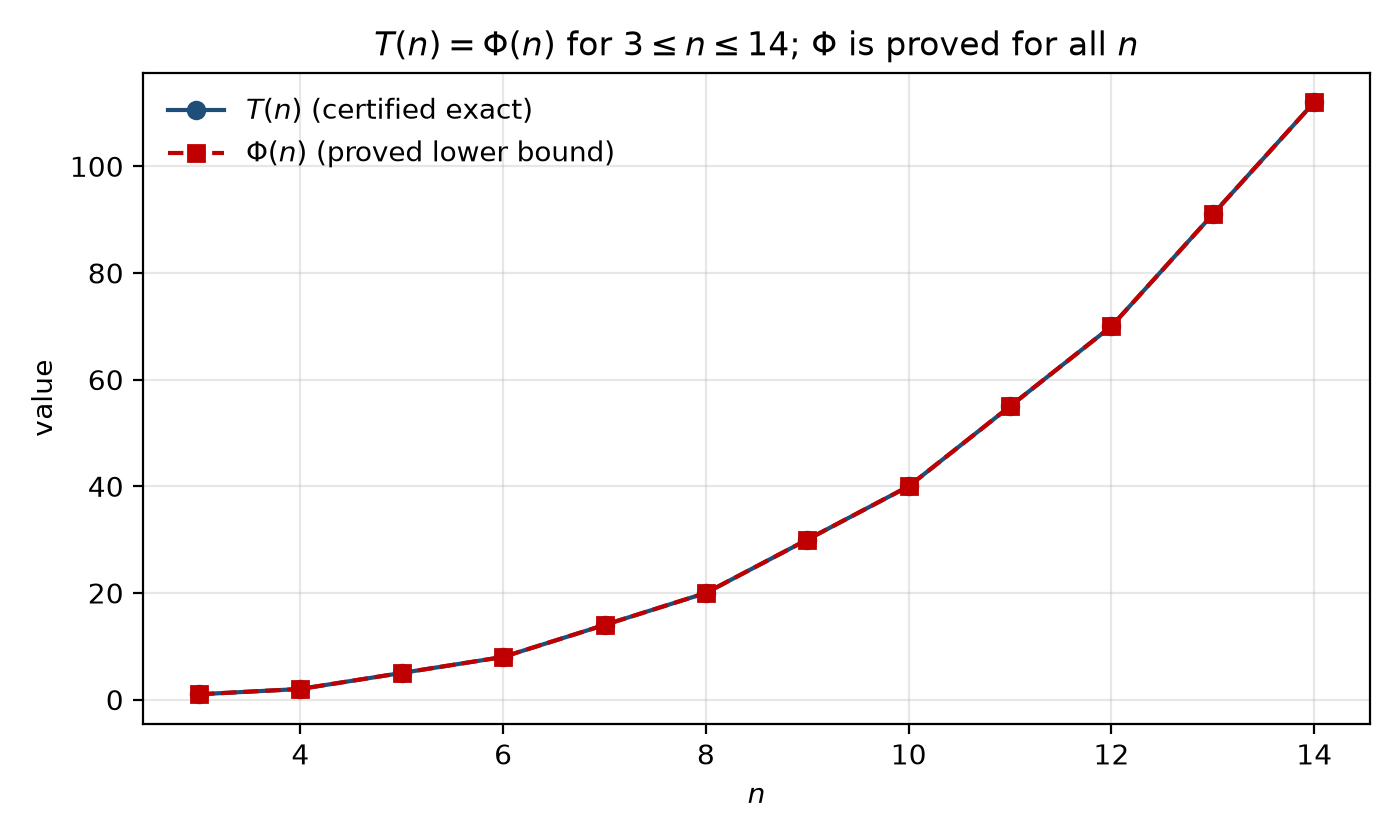
\includegraphics[width=0.86\textwidth]{F1_T_vs_Phi.png}
\caption{The exact values coincide with the proved lower bound wherever we can
compute them (Theorem~\ref{thm:exact}).}
\label{fig:exact}
\end{figure}

\begin{figure}[h]
\centering
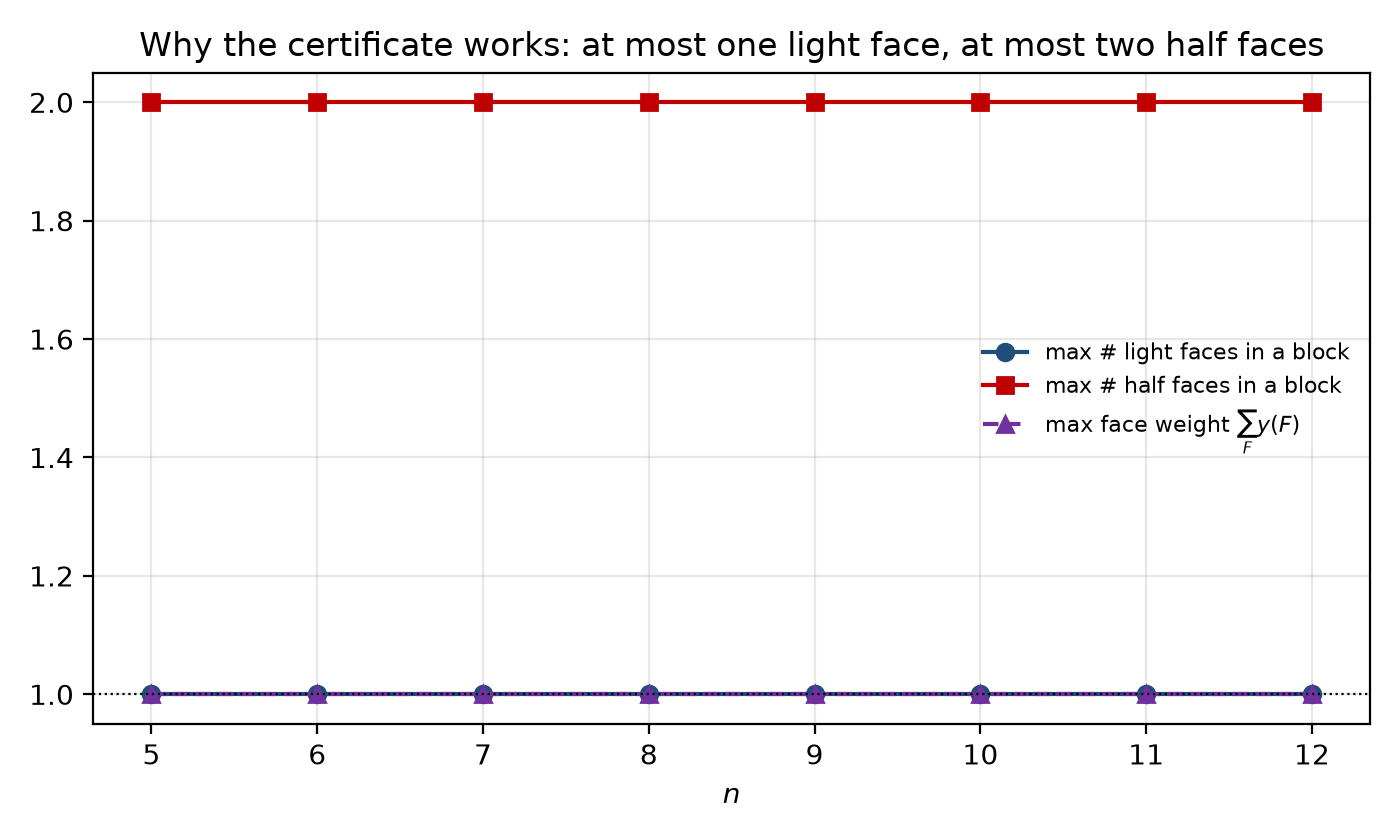
\includegraphics[width=0.86\textwidth]{F3_face_profiles.png}
\caption{Why the certificate works: any block has at most one light face and at
most two half faces, so its face weights sum to at most $1$ (Theorem~
\ref{thm:weightbound}).}
\label{fig:profiles}
\end{figure}

\begin{figure}[h]
\centering
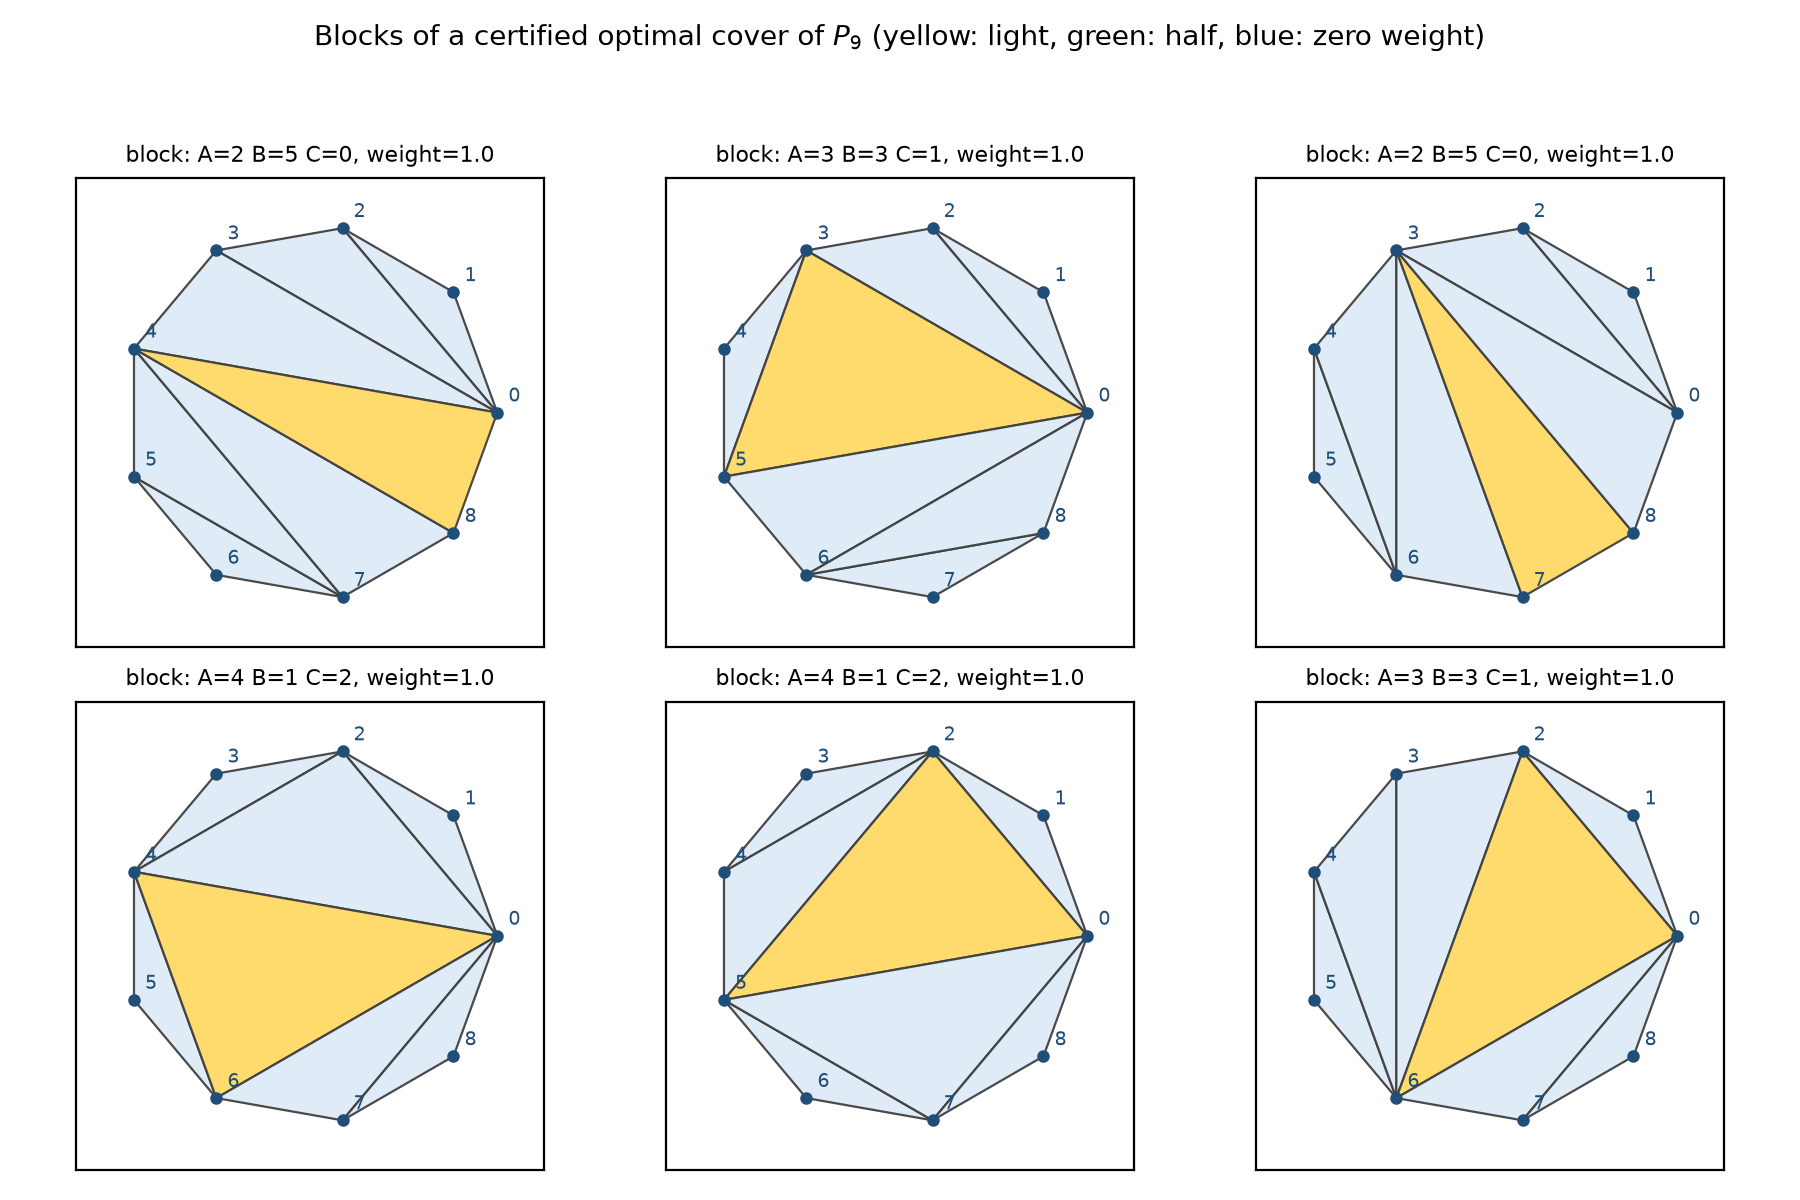
\includegraphics[width=0.86\textwidth]{F5_optimal_cover_P9.png}
\caption{Six blocks of a certified optimal triple cover of $\Pol_9$. Each block has
face weight exactly $1$: exactly one light face (yellow) and nothing else of
positive weight.}
\label{fig:cover}
\end{figure}

\section{Limitations}\label{sec:limits}

\begin{itemize}[leftmargin=1.4em]
\item The exact values are certified only for $n \le 14$. Beyond that the
      exponential number of blocks ($4^{n}$ up to polynomial factors) makes the
      MILP impractical; $n = 14$ already takes about $96$ seconds.
\item The general upper bound is open. We conjecture $T(n) = \Phi(n)$ but prove
      only the lower bound, the exact values up to $n = 14$, and the exact
      optimum $n$ of the type-$A$/$B$ sub-problem.
\item $\Phi(n)$ is a lower bound, not a proved asymptotic formula for $T(n)$; the
      claim $T(n) \sim n^3/24$ is part of Conjecture~\ref{conj:main}.
\item The certificate uses weights that were found with an LP solver for small
      $n$ and then proved directly; the proof is independent of the solver, but
      we do not claim the weight function is the unique optimal dual solution.
\item Only convex polygons are treated. Points in general position have a
      different face structure and the type-$A$/$B$/$C$ decomposition used here
      does not apply.
\item The two structural lemmas are proved for $n \ge 5$ and checked
      exhaustively only up to $n \le 13$.
\end{itemize}

\section{Conclusion}\label{sec:conclusion}

Covering every triple of a convex polygon by triangulations turns out to be a
genuinely hard covering problem: its minimum is cubic in $n$, while the naive
counting bound is quadratic, and the two classical decompositions of $K_n$ into
outerplanar pieces do not address it at all. We identified the mechanism behind
the true size: a single triangulation can realise at most one ``light'' triple,
in the sense of the largest cyclic gap between its vertices, and the total number
of light and half triples is exactly $\Phi(n) = n^3/24 - O(n)$. This yields a
sharp lower bound valid for all $n$, exact values for $n \le 14$ with machine
verification, and a precise description of what a general construction would
have to achieve.

\section*{Reproducibility}

\begin{verbatim}
pip install -e .
python -m pytest tests
python experiments/E1_exact_values.py --max-n 14
python experiments/E2_certificate.py
python experiments/E3_falsification.py --max-n 12 --restarts 9
python experiments/E4_upper_bounds_and_scaling.py
python experiments/E5_counting_formula_check.py
python experiments/make_figures.py
\end{verbatim}
Python $\ge 3.10$ with \texttt{numpy}, \texttt{scipy} (HiGHS is bundled),
\texttt{matplotlib}. Total runtime is a few minutes except \texttt{E1} with
$--\texttt{max-n} \ge 14$.

\begin{thebibliography}{9}
\bibitem{bernhartkaainen1979}
F.~Bernhart and P.~C. Kainen.
\newblock The book thickness of a graph.
\newblock \emph{J. Combin. Theory Ser. B}, 27(3):320--331, 1979.

\bibitem{buchbergerosipov1998}
K.~Buchberger and A.~Yu.~Osipov.
\newblock The thickness of the complete graph.
\newblock \emph{Combinatorica}, 18(1):39--46, 1998.

\bibitem{beinekeharary1965}
L.~W.~Beineke and F.~Harary.
\newblock Graph thickness.
\newblock \emph{J. Combin. Theory}, 2(3):149--151, 1965.

\bibitem{furedietal2020}
Z.~F\"uredi, D.~Mubayi, J.~O'Neill and J.~Verstra\"ete.
\newblock Extremal problems for pairs of triangles.
\newblock \emph{arXiv:2010.11100 [math.CO]}, 2020.

\bibitem{colbourndinitz}
C.~J.~Colbourn and J.~H.~Dinitz (eds.).
\newblock \emph{Handbook of Combinatorial Designs}.
\newblock Wiley-Interscience, 2007.

\bibitem{hiGHS}
Q.~Huangfu and J.~A.~J.~Hall.
\newblock Parallelizing the dual revised simplex method.
\newblock \emph{Math. Program. Comput. Sci.}, 10(1):119--142, 2018.
\end{thebibliography}

\appendix

\section{Algebra of the counting lemma}\label{app:counting}

With $s = n-3$ and $k = \lfloor s/2 \rfloor$ the counting lemma reduces to
evaluating
\[
  G(s,m) = \sum_{j=0}^{3} (-1)^j \binom{3}{j}\binom{s - j(m+1) + 2}{2},
  \qquad \binom{t}{2} = 0 \text{ for } t < 2.
\]

\emph{Odd case $n = 2M+1$.} Here $s = 2M-2$, $k = M-1$ and $k+1 = M$, so
\begin{align*}
G(2M-2, M-1) &= \binom{2M}{2} - 3\binom{M}{2} + 3\binom{0}{2} - \binom{-M}{2} \\
             &= M(2M-1) - \tfrac{3M(M-1)}{2} = \frac{M(M+1)}{2}.
\end{align*}
All light triples have weight $1$ and there are no half triples of positive
weight, so
\[
\sum_S y(S) = \frac{2M+1}{3}\cdot\frac{M(M+1)}{2}
            = \frac{M(M+1)(2M+1)}{6} = \sum_{j=1}^{M} j^{2} = \Phi(2M+1),
\]
the last step being the classical sum-of-squares identity.

\emph{Even case $n = 2M$.} Here $s = 2M-3$, $k = M-2$ and $k+1 = M-1$:
\begin{align*}
G(2M-3, M-2) &= \binom{2M-1}{2} - 3\binom{M}{2} + 3\binom{1}{2} - \binom{2-M}{2} \\
             &= (2M-1)(M-1) - \tfrac{3M(M-1)}{2} = \frac{(M-1)(M-2)}{2},\\
G(2M-3, M-1) &= \binom{2M-1}{2} - 3\binom{M-1}{2} + 3\binom{1}{2} - \binom{3-2M}{2} \\
             &= (2M-1)(M-1) - \tfrac{3(M-1)(M-2)}{2} = \frac{(M-1)(M+4)}{2}.
\end{align*}
Hence the number of light triples is
$\frac{2M}{3}\cdot\frac{(M-1)(M-2)}{2} = \frac{M(M-1)(M-2)}{3}$ and the number
of half triples is
$\frac{2M}{3}\cdot\frac{(M-1)\cdot 6}{2} = 2M(M-1)$, and therefore
\[
\sum_S y(S) = \frac{M(M-1)(M-2)}{3} + \frac{2M(M-1)}{2}
            = \frac{M(M-1)(M+1)}{3} = 2\binom{M+1}{3} = \Phi(2M).
\]

The formulas for the numbers of light and of half triples are verified against
brute force for $6 \le n \le 18$, and $\sum_S y(S) = \Phi(n)$ is verified for
$5 \le n \le 60$, by \texttt{experiments/E2\_certificate.py} and
\texttt{experiments/E5\_counting\_formula\_check.py}.

\section{Why the naive bounds fail}\label{app:capacity}

For completeness we record the counting bound that a covering design would give,
to make the gap explicit. A block is a face set of size $n-2$ contained in
$\binom{n}{3}$ triples, so the classical counting bound for $t = 3$ coverings is
\begin{equation}\label{eq:capacity}
  T(n) \ge \left\lceil \frac{\binom{n}{3}}{n-2} \right\rceil
        = \left\lceil \frac{n(n-1)}{6} \right\rceil .
\end{equation}
Using Proposition~\ref{prop:budget} one only has to cover the $C$-triples, which
gives
\[
T(n) \ge \frac{|\mathcal{C}_n|}{\lfloor n/2 \rfloor - 2}
      = \frac{n(n-4)(n-5)}{6\,(\lfloor n/2 \rfloor - 2)},
\]
i.e.\ $n^2/3 + O(n)$ for even $n$ and asymptotically the same for odd $n$.
Both bounds are quadratic, whereas $\Phi(n)$ is cubic: for $n = 20$ they read
$63$ and $132$ while $\Phi(20) = 330$. Theorem~\ref{thm:main} is therefore not a
refinement of the counting argument but a different phenomenon.

\end{document}